\cotefile{71}
\scanpage{21}\mspage{I}
Le théorème de Jordan et l'existence de trois bons sommets pour un polygone \tikz[baseline=(a.base)]{\node[inner sep=1pt] (a) {de $\mathbb{R}^{2}$.};\draw[thin,gray,rotate around={8:(a.center)}] (a.center) ellipse (0.65cm and 0.30cm);}\inserted{plan}

\hspace*{\fill}Carlos C.~\unsure{Contou|Coutou}-Carrère\hspace*{\fill}

\margin{$\bullet$}On se propose de prouver les deux théorèmes \unsure{suivantes|suivants} :

\uline{Théorème} 1 (Jordan). Tout polygone $\Gamma$ est un \unsure{$J$|$j$}-polygone (cf. def 1)

\uline{Théorème} 2 (Dehn (?) non-publié). Si $\Gamma$ est un polygone, il existe au moins trois bons sommets (cf. def.\hspace{1em}) dont deux au moins sont tels que les triangles correspondants soient \unsure{inteieurs|interieurs|intérieurs}, i.e. contenus dans $\mathrm{int}_{\Gamma}\cup\Gamma$ (cf. def 2).

1- \uline{Preliminaires}

\margin{$\bullet\ \bullet$}On entend par polygone la réalisation \uline{géom}étrique dans \uline{$\mathbb{R}^{2}$} d'un \margin{$\bullet$}polygo\uline{ne abs}trait, connexe\inserted{et non vide}. Si $\Gamma$ est un polygone on dénote par \margin{$\bullet$}$S(\Gamma)$ (resp. $A(\Gamma)$) l'ensemble des sommets (resp. arêtes) gé\uline{ometriq}\unsure{ues} de $\Gamma$.

\margin{$\cdot\quad\cdot$}Le terme ar\uline{c de} polygone désigne la réalisation \uline{géo}metrique dans $\mathbb{R}^{2}$ d'un 1-complexe connexe\unsure{$\langle$|,} \margin{\unsure{or.|ou.}?}tel que chaque sommet soit incident à 1 ou à 2 arêtes, et tel qu'il existe exactement 2 sommets qui sont incidents à une seule arête (pas néc. la même).

On appelle extrémités \unsure{d'un|deun} arc de polygone les points de $\mathbb{R}^{2}$ qui correspondent à ces deux sommets. Si $\Gamma_{xy}$ est un arc de polygone d'\unsure{extremités|extrémités} $x,y$ on dénote par $S(\Gamma_{xy})$ (resp. $A(\Gamma_{xy})$) l'ensemble de ses sommets (resp. arêtes) géometriques.

\margin{$\bullet$}Par $\Gamma$ (resp. $\Gamma_{xy}$) on dénote \uline{aussi} l'ensemble \inserted{de $\mathbb{R}^{2}$} sous jacent à $\Gamma$ (resp. $\Gamma_{xy}$) si $\Gamma$ \deleted{est} (resp. $\Gamma_{xy}$) est un polygone (resp. arc de polygone).

\tikz[baseline=(r.base)]{\node[inner sep=1pt] (r) {\uline{Remarque 1}};\draw[dashed,gray,line width=.2pt] ([xshift=-1pt,yshift=1pt]r.north east)..controls ([yshift=5pt]r.north) and ([xshift=-3pt,yshift=4pt]r.north west)..([xshift=-3pt]r.west)..controls ([xshift=-3pt,yshift=-4pt]r.south west) and ([yshift=-3pt]r.south)..([xshift=-2pt,yshift=-2pt]r.south east);}. Si $x,y$ $(x\ne y)$ est un couple de points d'un polygone $\Gamma$ il existe \margin{$\cdot$}un seul co\uline{up}le d'arcs de polygone $\Gamma^{1}_{xy}$ et $\Gamma^{2}_{xy}$ d'\unsure{extremités|extrémités} $x,y$\unsure{.} tels que : $\mathrm{I})\quad S(\Gamma^{i}_{xy})-\{x,y\}\subset S(\Gamma),\ i=1,2$ ; $\mathrm{II})$ si $\unsure{s|z|g}$ \deleted{$\unsure{(\Gamma_{xy})|(x,y)}$}
\margin{\unsure{faut|faux}}
% slanted
\par\noindent$\unsure{\subset|c}$
% archive sheet number: 20

\scanpage{22}
\noindent\begin{minipage}[t]{.30\linewidth}
\figure{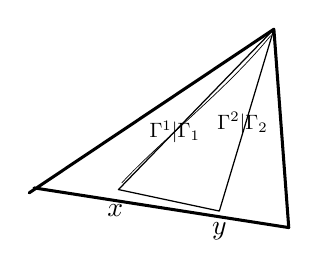
\begin{tikzpicture}[x=.021cm,y=-.021cm,line join=round,line cap=round]
\draw[line width=1.1pt] (0,102)--(148,3)--(157,123)--(3,99);
\draw[line width=.45pt] (148,3)--(54,100)--(115,113)--cycle;
\draw[line width=.25pt] (56,96)..controls (79,71) and (119,40)..(146,7);
\node[below] at (52,103) {$x$};
\node[below] at (115,114) {$y$};
\node[inner sep=0pt,scale=.75] at (88,65) {$\unsure{\Gamma^{1}|\Gamma_{1}}$};
\node[inner sep=0pt,scale=.75] at (129,60) {$\unsure{\Gamma^{2}|\Gamma_{2}}$};
\end{tikzpicture}}
\end{minipage}\hfill
\begin{minipage}[t]{.67\linewidth}
\small
\[
\left\{\begin{aligned}
\Gamma^{1}_{xy}\cap\Gamma^{2}_{xy}&=\{x,y\}\\
\Gamma^{1}_{x,y}\cup\Gamma^{2}_{x,y}&=\Gamma\\
S'(\Gamma^{1}_{\unsure{x|xx}y})\cup S'(\Gamma^{2}_{xy})&=S(\Gamma)\setminus\{x,y\}\unsure{\cap S(\Gamma|S(\Gamma}
\end{aligned}\right.
\]
\uline{NB} Ce n'est pas le \uline{couple} $(\Gamma^{1}_{xy},\Gamma^{2}_{xy})$ qui est \unsure{déterminé} de \unsure{façon} unique mais l'\uline{ens} $\{\Gamma^{1}_{xy},\Gamma^{2}_{\unsure{x,y|xy}}\}$
\end{minipage}

a) op. de \unsure{rajouter|rajout de} \unsure{sommet|sommets}

b) op. de \unsure{division} d'un \unsure{polygone} (par 2 \unsure{sommets|sommet} distincts) en deux lignes polygonales (op. \unsure{inverse} : \unsure{recollement} de 2 lignes polygonales \unsure{ayant} \unsure{$=$|mêmes} extrémités).

\figure{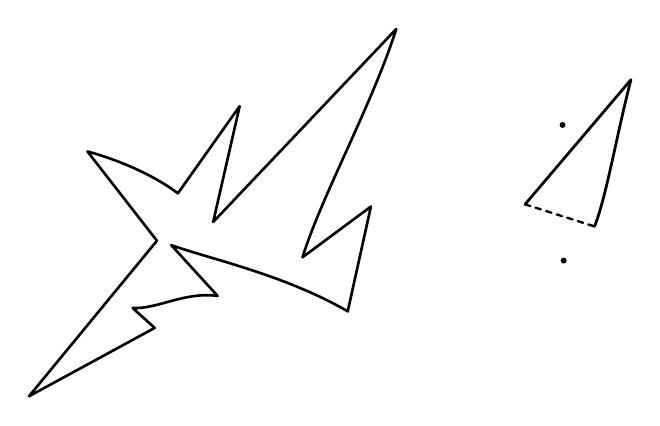
\begin{tikzpicture}[x=.014cm,y=-.014cm,line join=round,line cap=round]
\draw[line width=.95pt] (53,112)..controls (89,122) and (118,137)..(135,150)--(191,71)--(167,176)--(333,1)..controls (311,70) and (265,153)..(248,208)--(310,162)--(289,257)..controls (232,224) and (166,210)..(129,197)--(171,243)..controls (141,239) and (117,255)..(94,254)--(114,272)--(0,334)--(116,193)--cycle;
\begin{scope}[xshift=6.3cm]
\draw[line width=1pt] (0,160)--(96,47)..controls (83,97) and (74,152)..(63,180);
\draw[dash pattern=on 2pt off 2pt,line width=.85pt] (0,160)--(63,180);
\fill (34,88) circle[radius=2.7];
\fill (35,211) circle[radius=2.7];
\end{scope}
\end{tikzpicture}}
% archive sheet number: 21

\scanpage{23}\mspage{II}
$\in S(\Gamma)$ appartient à $\Gamma^{i}_{xy}$ alors $s\in S(\Gamma^{i}_{xy}),\ i=1,2$.
\margin{\tikz[x=.06cm,y=.06cm]{\draw (1,0)--(0,2)--(.2,3)--(-.5,4)--(0,5)--(-.4,6)--(.5,7)--(-.3,7.8)--(-.8,7.2);}}

Si $\Lambda^{1}_{xy}$ et $\Lambda^{2}_{xy}$ sont deux arcs de polygone vérifiant \margin{$\bullet$}$\Lambda^{1}_{xy}\cap\Lambda^{2}_{xy}=\{x,y\}$ on peut obtenir par \unsure{récollement|recollement} selon $\{x,y\}$ un polygone $\Lambda$ de façon évidente.

\margin{\unsure{bis|dir}}%
\margin{$\bullet$}\uline{Definition 1}. On dit \unsure{que'un|qu'un} polygone $\Gamma$ est un $J$-polygone, ou bien que $\Gamma$ est de Jordan si $\Gamma$ vérifie :

a) $\mathbb{R}^{2}-\Gamma=U\cup V$ avec $U$ et $V$ connexes, $U$ relativement compact et \uline{$\overline{V}$ non-compact}, On pose $U=\mathrm{int}\,\Gamma$, $V=\mathrm{ext}\,\Gamma_{\unsure{\bullet|,|x}}$ ;
\margin{$V$\,! \unsure{non rel. compact}}
% slanted

b) Si $D_{x}$ est un disque de centre $x\in\Gamma$ qui ne coupe que les arêtes de $\Gamma$ auxquelles $x$ appartient (deux au plus), alors $D_{x}-D_{x}\cap\Gamma=U'\unsure{\cup|\mathbin{\dot\cup}}V'$, avec $U'\subset\mathrm{int}\,\Gamma$ et $V'\subset\mathrm{ext}\,\Gamma$ connexes\inserted{(i.e. les 2 comp. conn. de $D_{x}-D_{x}\cap\Gamma$ \deleted{\unsure{appartiennent}} \inserted{\unsure{sont contenues}}, l'une dans $\mathrm{int}\,\Gamma$)\unsure{,|;} l'autre \unsure{dans} $\mathrm{Ext}\,\Gamma$\unsure{)|,}}.
\margin{non \uuline{\unsure{vides|vide}}\,!}
% slanted

\margin{style}%
\uline{Remarque} 2 On voit qu'il suffit qu'un seul disque \deleted{tel} qui ne coupe $\Gamma$ \deleted{ailleurs} que dans les \deleted{\illegible{1}} arêtes auxquelles $x$ appartient vérifie la propriété de b), pour que tout \unsure{autre} \inserted{ayant cette \deleted{\unsure{mê|m}} même propriété} disque \inserted{la} vérifie \inserted{(car \inserted{si $D_{x}\subset\unsure{D'_{x}|D_{x'}}$,} $\unsure{\pi_{0}|\Pi_{0}}(D_{x}-D_{x}\cap\Gamma)$ $\unsure{\longrightarrow|-}$ $\pi_{0}(D'_{x}-\unsure{D'_{\bullet}|D'_{x}}\cap\Gamma)$ est bijectif)}

On pose $R_{\Gamma}=\mathrm{int}\,\Gamma\cup\Gamma$.

\margin{$\cdot$}\uline{Definition} 2. On dit que $s\in S(\Gamma)$ est un \uline{bon sommet} de $\Gamma$ s'il \margin{\unsure{,}}n'est pas \unsure{colineaire|colinéaire} avec les deux sommets $s',s''$ qui sont adjacents à $s$, et si le triangle de sommets $s,s',s''$ ne contient aucun sommet de $\Gamma$ à l'interieur. \inserted{(On \uline{suppose connue} la \uline{notion} de \unsure{interieur|intérieur} ou de \unsure{exterieur|extérieur} d'un triangle\unsure{.)|).}}

\margin{vague}%
\inserted{\uline{Déf 3}\unsure{?|.}}

% The marginal pen strokes flank the two paragraphs on the bottom strip.
\margin{\tikz[x=.1cm,y=.1cm]{\draw (0,0)..controls (.2,1.2) and (1.3,.4)..(1.5,1.4);}}%
\margin{\rule{.35pt}{1em}}%
Si $E$ est une partie de $\mathbb{R}^{2}$ \inserted{et $s,s'\in\mathbb{R}^{2}$,} on dit que $s'$ est $E$-visible de $s$ si le segment \margin{\tikz[x=.1cm,y=.1cm]{\draw (0,0)--(0,1) (0.4,.65)--(1.5,.65)--(1.5,0);}}ouvert $]s,s'[$ est contenu dans $E$ \deleted{$\unsure{(s,s'\in\mathbb{R}^{2})|/s,s'\in\mathbb{R}^{2}/}$}.

\margin{\rule{.35pt}{1em}}Si $\Gamma$ est un $J$-polygone on dit que $s'$ est visible de $s$ de l'\unsure{exterieur|extérieur} \inserted{(resp. \unsure{interieur|intérieur})} de $\Gamma$ si $s'$ est $\mathrm{ext}\,\Gamma$ (res. $\mathrm{int}\,\Gamma$) - visible de $s$.\margin{\rule{.35pt}{1em}}
% archive sheet number: 22

\scanpage{24}
\figure{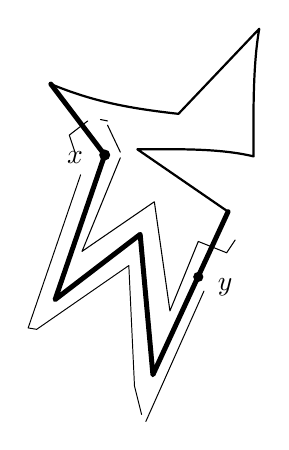
\begin{tikzpicture}[x=.018cm,y=-.018cm,line join=round,line cap=round]
\draw[line width=.8pt] (22,39)..controls (51,51) and (76,56)..(112,60)--(169,0)..controls (164,28) and (165,68)..(165,90)..controls (140,84) and (109,85)..(83,85)--(147,129);
\draw[line width=1.8pt] (22,39)--(60,89)--(25,191)--(85,145)--(94,244)--(147,129);
\draw[line width=.38pt] (48,65)--(35,75)--(39,87) (57,64)--(62,65) (62,68)--(71,87);
\draw[line width=.38pt] (71,91)--(44,157)--(95,122)--(106,199)--(126,150)--(146,158)--(152,149);
\draw[line width=.35pt] (43,103)--(6,211)--(12,212)--(77,167)--(81,252)--(86,272);
\draw[line width=.36pt] (89,277)--(130,185);
\fill (60,89) circle[radius=3.9];
\fill (126,175) circle[radius=3.6];
\node[inner sep=0pt] at (39,91) {$\unsure{x}$};
\node[inner sep=0pt] at (145,182) {$y$};
\end{tikzpicture}}

% The lower strip shows through horizontally reversed. The direction is restored
% here to read the three lines. Two lines carry a stroke through their text.
\margin{\tikz[x=.07cm,y=.07cm]{\draw (0,0)--(.1,-.6) (.15,-1.4)--(.1,-2.8);}}%
\uline{\unsure{Definition|Définition}} 3. Si $\Gamma$ est un polygone et $s,s'\in\mathbb{R}^{2}-\Gamma$ on dit que
\deleted{$s$ est visible de $s'$ ou bien que le couple \inserted{\unsure{de points} $s,s'$} est mutuellement visible si}

\margin{\tikz[x=.07cm,y=.07cm]{\draw (0,0)--(.12,-1) (.1,-1.45)--(-.14,-2.8);}}%
\margin{\tikz[x=.07cm,y=.07cm]{\draw (.15,0)..controls (.35,-.4) and (0,-.8)..(-.1,-1.2) (-.1,-1.5)..controls (0,-1.9) and (.1,-2.25)..(-.1,-2.7);}}%
\[
\deleted{\unsure{[s,s']|]s,s'[}\unsure{-|=}\{s,s'\}\unsure{\subset|\in}\mathbb{R}^{2}-\Gamma.}
\]
% archive sheet number: 23

\scanpage{25}\mspage{III}
\margin{\tikz[x=.08cm,y=.08cm]{\draw (0,0)..controls (1,1.1) and (2.1,1.9)..(1.4,2.8);}}%
\uline{Lemme I}. Soit $\Gamma$ un $J$-polygone et $x,y\in\Gamma$ \inserted{$x\ne y$} ; si $\Gamma^{\unsure{*|\star}}_{xy}$ est l'un de deux arcs de polygone \unsure{réliant|reliant} $x$ à $y$, décrit dans la Remarque 1, \margin{!\ \tikz[x=.07cm,y=.07cm]{\draw (0,0)..controls (.4,2) and (1.7,2.4)..(1.5,3.4);}}il \uline{existe un système} fondamental \inserted{$\unsure{\beta|B}$} de voisinages \deleted{$\beta$} \inserted{ouverts} de $\Gamma^{*}_{xy}$ tel que $V\in\beta$ vérifie :
\margin{$\cdot$}
\[
\begin{aligned}
&V\cap\mathrm{int}\,\Gamma\quad\text{et}\quad V\cap\mathrm{ext}\,\Gamma\quad\text{sont connexes (donc}\\
&V-V\cap\Gamma=(V\cap\mathrm{int}\,\Gamma)\cup(V\cap\mathrm{ext}\,\Gamma)\ \text{a deux composantes connexes)}
\end{aligned}
\]

\margin{!}\uline{Demonstration}. gr\uline{âce à l'axiom du c}hoix il suffit de prouver que si $U$ est un voisinage \uline{de $\Gamma$}, \margin{!\\$\Gamma_{xy}$}il existe un voisinage ouvert $V\subset U$ satisfaisant \inserted{à} la condition de l'ennoncé. Pour chaque $z\in\Gamma_{xy}$ on choisit un disque \inserted{ouvert} $D_{z}\subset U$ et satisfaisant b) de la definition 1\unsure{,|3|;} par rapport a $\Gamma$. Il est clair que $\{D_{z}\}_{\inserted{z\in\Gamma_{xy}}}$ est un \unsure{récouvrement|recouvrement} ouvert de l'ensemble compact $\Gamma_{xy}$. Soit donc un sous-récouvrement fini $\{D_{z_{i}}\}^{n}_{i=1}$ de $\Gamma_{xy}$.

Soit $I_{i}$ l'intervalle \inserted{ouvert ou semiouvert de $\Gamma_{xy}$} \unsure{decoupé|découpé} par $D_{z_{i}}$, i.e. \inserted{\tikz[baseline=(f.base)]{\node[inner xsep=.12em,inner ysep=.12ex] (f) {$\deleted{\unsure{I|F}}\Gamma_{xy}\cap D_{z_{i}}=I_{i}.$}; \draw[line width=.5pt] ([xshift=-.65em]f.south west)--(f.south west)--(f.north west); \draw[line width=.5pt] ([xshift=.30em,yshift=.35ex]f.north west)--([yshift=.65ex]f.north east)..controls ([xshift=.12em,yshift=.58ex]f.north east) and ([xshift=.15em]f.south east)..([xshift=.23em]f.south east)--([xshift=.45em]f.south east);}} On observe que si $I_{i}\cap I_{j}\ne\unsure{\phi|\emptyset}$ alors $D_{z_{i}}\cap D_{z_{j}}\cap\mathrm{int}\,\Gamma\ne\phi$. Cela permet de montrer que si $z',z''\in\bigcup\limits_{i=1}^{n}D_{z_{i}}\cap\mathrm{int}\,\Gamma$ il existe une suite :

$D_{z_{i_{1}}}\cap\mathrm{int}_{\Gamma},\ \ldotp\;\ldotp\;\unsure{-|\ldotp}\,{-},\ D_{z_{i_{m}}}\cap\mathrm{int}\,\Gamma$ d'ouverts connexes (par le choix de chaque $D_{z}$) tels que $D_{z_{i_{\unsure{\alpha|a}}}}\cap D_{z_{i_{\alpha+1}}}\cap\mathrm{int}\,\Gamma\ne\phi$ pour $1\le\alpha\le m-1$, et $z'\in D_{z_{i_{1}}}\cap\mathrm{int}_{\Gamma},\ z''\in D_{z_{i_{m}}}\cap\mathrm{int}\,\Gamma$. Ces deux propriétés \unsure{verifiées|vérifiées} par $\bigcup\limits_{i=1}^{n}D_{z_{i}}\cap\mathrm{int}\,\Gamma$ suffisent à prouver la connexité de $\bigcup\limits_{i=1}^{n}D_{z_{i}}\cap\mathrm{int}\,\Gamma$.

\margin{!\ $\cdot$}\deleted{\unsure{Une|Un}} Le même argument prouve (qui\uline{tte à changer $\mathrm{int}\,\Gamma$ par $\mathrm{ext}\,\Gamma$}) que $\bigcup\limits_{i=1}^{n}D_{z_{i}}\cap\mathrm{ext}\,\Gamma$ est connexe. Par conséquent il suffit de prendre $V=\bigcup\limits_{i=1}^{n}D_{z_{i}}$, Cela montre le lemme.

\margin{$\bullet$\quad\uline{?}}On\textsuperscript{\unsure{$*$}} utilise le fait, \uline{sans le dire}, que \deleted{tout couple de} \inserted{deux} points $x,y$ \deleted{\unsure{de|un}} \inserted{d'un} ouvert connexe de $\mathbb{R}^{2}$ peu\deleted{t}\inserted{vent} être reliés par un arc de polygone.
% archive sheet number: 24

\scanpage{26}
% Cancelled block at the foot of the scan, written upside down.
\deleted{Lemme I. Soit $\Gamma$ un $J$-polygone et $x,y\in\Gamma$, si $\Gamma^{1}_{xy}$ est l'un de deux arcs de polygone réliant $x$ à $y$, il existe un système fondamental $\unsure{\beta|B}$ de voisinages ouverts \inserted{de $\Gamma^{1}_{xy}$}, tel que si $V_{\boxed{\unsure{\Gamma_{xy}|xy}}}\in\beta$ il vérifie}
% archive sheet number: 25

\scanpage{27}\mspage{IV}
2 - \uline{Rappel sur les sous-ensembles convexes de $\mathbb{R}^{2}$}.

\margin{!}\uline{Lemme II}. Si $A$ est une partie \inserted{\uline{finie}} de $\mathbb{R}^{2}$ contenant trois points affinement independants, il existe un polygone et un seul $\Gamma$ tel qu'il n'y ait pas trois sommets consecutifs colineaires \inserted{de $\Gamma$}, et \deleted{de façon} que l'ensemble sous-jacent à $\Gamma$ soit égal a $E(A)-\overset{\circ}{E(A)}$ ($E(A)=$ enveloppe convexe de $A$).

On a aussi $S(\Gamma)\subset A$.

\margin{\unsure{jargon}\\\tikz[x=.12cm,y=.12cm,baseline=0pt]{\draw (0,0)--(.12,-.10)--(.85,3.3);}\quad ?\\$\cdot$}%
% slanted
\uline{Demonstration} (\unsure{Esquisse|Esquissè|Esquissé}) Cela résulte du fait que $E(A)=\tikz[baseline=(q.base)]{\node[inner sep=1pt] (q) {$\cap$};\draw[rotate around={-12:(q.center)}] (q.center) ellipse (.17cm and .35cm);}$ demi espaces fermés correspondants à un ensemble de droites uniquem\uline{ent determinées par} la donnée de $A$, On remarque aussi que $S(\Gamma)=$ \inserted{ens. des} points \unsure{extremaux|extrémaux} de $E(A)$.

\margin{!!!\\\unsure{partie polyédral conv.|partie polyédrale conv.}}%
% slanted
\uline{Convention} : Le mot ensemble convexe désigne \uline{pour nous} l'enveloppe convexe d'un ensemble fini de points dans $\mathbb{R}^{2}$. \inserted{Soit $\unsure{\mathbb{C}|C}$ un \uline{ensemble convexe},} Si l'\unsure{interieur|intérieur} est non-vide on munit $\partial\mathbb{C}=\mathbb{C}-\overset{\circ}{\mathbb{C}}$ de la structure de polygone décrite dans le lemme II. Il est clair qu'un \uline{ensemble convexe} $\mathbb{C}$ est compact et \inserted{par conséquent} $\partial\mathbb{C}=\mathbb{C}-\overset{\circ}{\mathbb{C}}$ aussi.
\margin{\unsure{intervertir|intervention} \unsure{avec} lemme II ! C'est une \unsure{salade}\ldots}

\uline{Lemme III}. Si $s,s'\in\partial\mathbb{C}$, $\overset{\circ}{\mathbb{C}}\ne\unsure{\phi|\emptyset}$, sont deux sommets consecutifs, la droite \deleted{$d$ qui} \inserted{$d$ qu'ils} déterminent partage $\mathbb{R}^{2}$ en deux demi-espaces fermés dont l'un contient $\overset{\circ}{\mathbb{C}}$.

\margin{?\quad ?\\\unsure{vis}\\\unsure{1|i}}%
\uline{Demonstration} : Cela est trivial quand on exprime $\mathbb{C}$ comme intersection de demi-espaces, si l'on tient compte que $\overset{\circ}{\mathbb{C}}$ est l'intersection des demi espaces ouverts correspondants, et qu'une \unsure{arète|arête} de $\partial\mathbb{C}$ est toujours contenue dans un \uline{tel} demi-espace, c.q.f.d.

\uline{Lemme IV}. Soit $\mathbb{C}$ un \uline{ensemble convexe} à interieur non vide. Si $x\notin\mathbb{C}$ il existe au moins un point $y\in\mathbb{C}-S(\partial\mathbb{C})$ tel que $y$ est $(\mathbb{R}^{2}-C)$-visible de $x$.

\uline{Démonstration} : Choisissons $z\in\overset{\circ}{\mathbb{C}}$ tel que la droite determinée par $x$ et par $z$ \deleted{coupe $\partial\mathbb{C}$} ne contienne aucun sommet de $\partial\mathbb{C}$ (cela est possible car il n'y a qu'un nombre fini de Sommets). Comme $d\cap\mathbb{C}$ est un convexe fermé de $d$ à interieur \inserted{(relatif)} non-vide il est de la forme $d\cap C=[z_{1},z_{2}]$, $z_{1}\ne z_{2}$, il suffit de prendre $y$ \deleted{$\unsure{=y_{1}|=z_{1}}$} egal au point de $[z_{1},z_{2}]$ qui realise le minimum de la \unsure{distence|distance} de $x$ a $[z_{1},z_{2}]$, \unsure{c.q-f-d.|c.q.f.d.}
\margin{!}
% archive sheet number: 26

